\chapter{Estado del arte}\label{chap:3estadodelarte}

En este capítulo se lleva a cabo un breve análisis de algunas implementaciones, tecnologías y plataformas que usan IPFS 
y cumplen parcial o completamente con los objetivos del proyecto.

Como se ha visto en el apartado anterior existen una gran cantidad de herramientas y proyectos
que usan IPFS como base para sus sistemas. Pese a esto en el contexto de archivos compartidos, solo existen
algunos proyectos interesantes que merece la pena analizar:

\section{Peergos}

Peergos es con una plataforma web para subir archivos y compartirlos con otros usuarios. Cuenta con un sistema de
almacenamiento y comunicación descentralizado y seguro que utiliza criptografía y la red IPFS. Como se puede observar en la
figura \ref{fig:peergos} Peergos proporciona una interfaz web para guardar,
compartir y editar archivos, fotos, vídeos, mensajes y otros datos de forma privada y sin intermediarios. Peergos garantiza que
solo los usuarios autorizados puedan acceder a sus datos, y que nadie pueda espiar o censurar su actividad en línea. Es una
plataforma de código abierto y se puede ejecutar en cualquier dispositivo compatible con Java \cite{PeergosPeergosP2p}.

Este proyecto se encuentra en fase de desarrollo, aunque es un producto completo que además ofrece planes de almacenamiento
como si de un proveedor en la nube se tratara. Esto es posible ya que al ser IPFS una red global,
cualquier nodo de la red puede mantener \textit{pinneados} (disponibles) los bloques que se deseen, y por tanto
ofrecer un servicio de almacenamiento. En este caso Peergos ofrece un servicio de almacenamiento de pago, es decir,
que tienen una serie de nodos en la red que mantienen pinneados los bloques de datos de los usuarios que pagan por el servicio.

\begin{figure}[H]
    \centering
    \small
    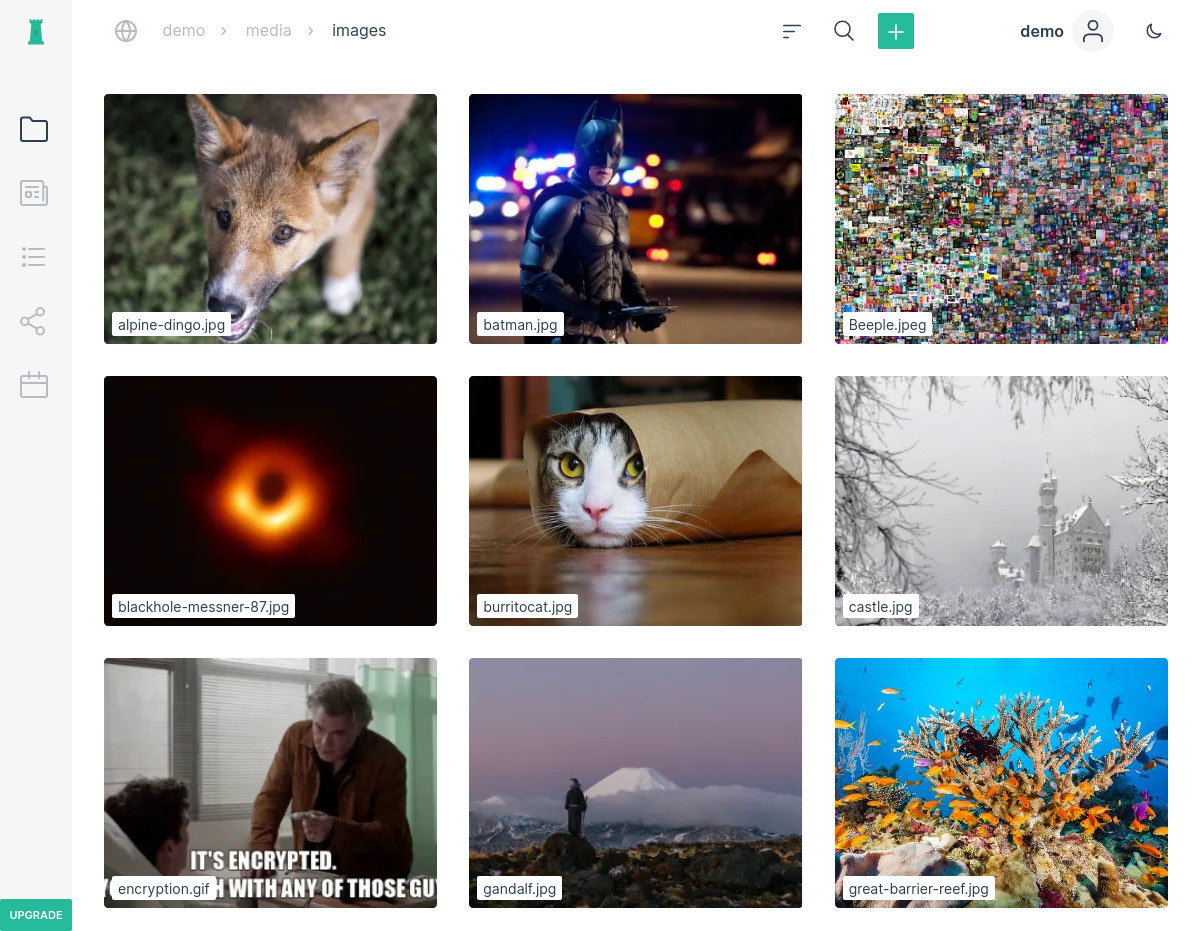
\includegraphics[width=0.8\linewidth]{images/peergos.jpg}
    \caption{Plataforma web de Peergos}
    \label{fig:peergos}
\end{figure}

Otro aspecto de gran interés es el sistema registro de usuarios. Las claves públicas y los nombres de usuario se almacenan en una estructura de datos global de solo adición,
con los  nombres asignados por orden de llegada. Esto requiere consenso para garantizar la singularidad de los nombres de usuario.
Aquí es también donde se almacena el ID del nodo IPFS del servidor (o servidores) responsables de sincronizar las escrituras del
usuario. El problema de la implementación realizada por Peergos es que se necesita de uno o varios servidores centralizado
que denominan \textit{Corenode} que mantienen y sirven este registro para los usuarios.

Este registro es en sí la base de datos de usuarios, la autenticación se maneja mediante un sistema de clave pública-privada
guardada en el navegador del usuario. Se usa una contraseña definida por el usuario para el acceso a la cuenta.

Peergos es una plataforma muy completa y que ofrece una gran cantidad de funcionalidades que escapan del alcance de este proyecto.
Se puede considerar esta plataforma como referencia del potencial de IPFS, y aunque no es perfecta y tiene sus limitaciones, es un buen ejemplo de lo que se puede lograr con esta tecnología.

\section{Filecoin}

Filecoin\cite{filecoinDecentralizedStorageNetwork} es una plataforma de almacenamiento descentralizado en la nube basada en
blockchain. La plataforma utiliza su propia criptomoneda,llamada Filecoin (FIL), para facilitar e incentivar las transacciones dentro
de la red.

Filecoin no está dirigido a consumidores (usuarios de a pie) ya que realmente es un mercado para proveedores de almacenamiento en la nube. Puede llegar
a ser de interés para el futuro de este proyecto ya que se podría integrar el sistema con Filecoin para ofrecer un servicio parecido
a un proveedor de almacenamiento en la nube, pero con distintos proveedores que compiten entre sí para ofrecer el mejor servicio.

\section{Sailplane}

Sailplane se describe como una plataforma para \textit{'Compartir archivos de forma colaborativa punto a punto en el navegador'}.

Sailplane, al igual que este proyecto, usa OrbitDB como el componente central de sus sistema\footnote{Este proyecto fue descubierto
    hacia el final del desarrollo de este trabajo de fin de grado por lo que este hecho es más bien una casualidad.}.
Como ya se ha explicado previamente, OrbitDB es una base de datos distribuida. Sailplane implementa un backend de almacenamiento
conocido como un \textit{store}. Un store en OrbitDB se refiere a una instancia de una base de datos individual que se sincroniza
automáticamente con otros stores del mismo tipo mediante la red IPFS.

Sailplane ha implementado su propio store llamado \textit{orbit-db-fsstore}\cite{TabcatOrbitdbfsstoreCustom}. Este representa
un sistema de ficheros montado sobre OrbitDB que se puede sincronizar con otras instancias de la base de datos, lo que permite
mantener y compartir un sistema de ficheros sincronizado entre varios usuarios. Este sistema de archivos se puede encriptar aunque no es necesario.

\begin{figure}[H]
    \centering
    \small
    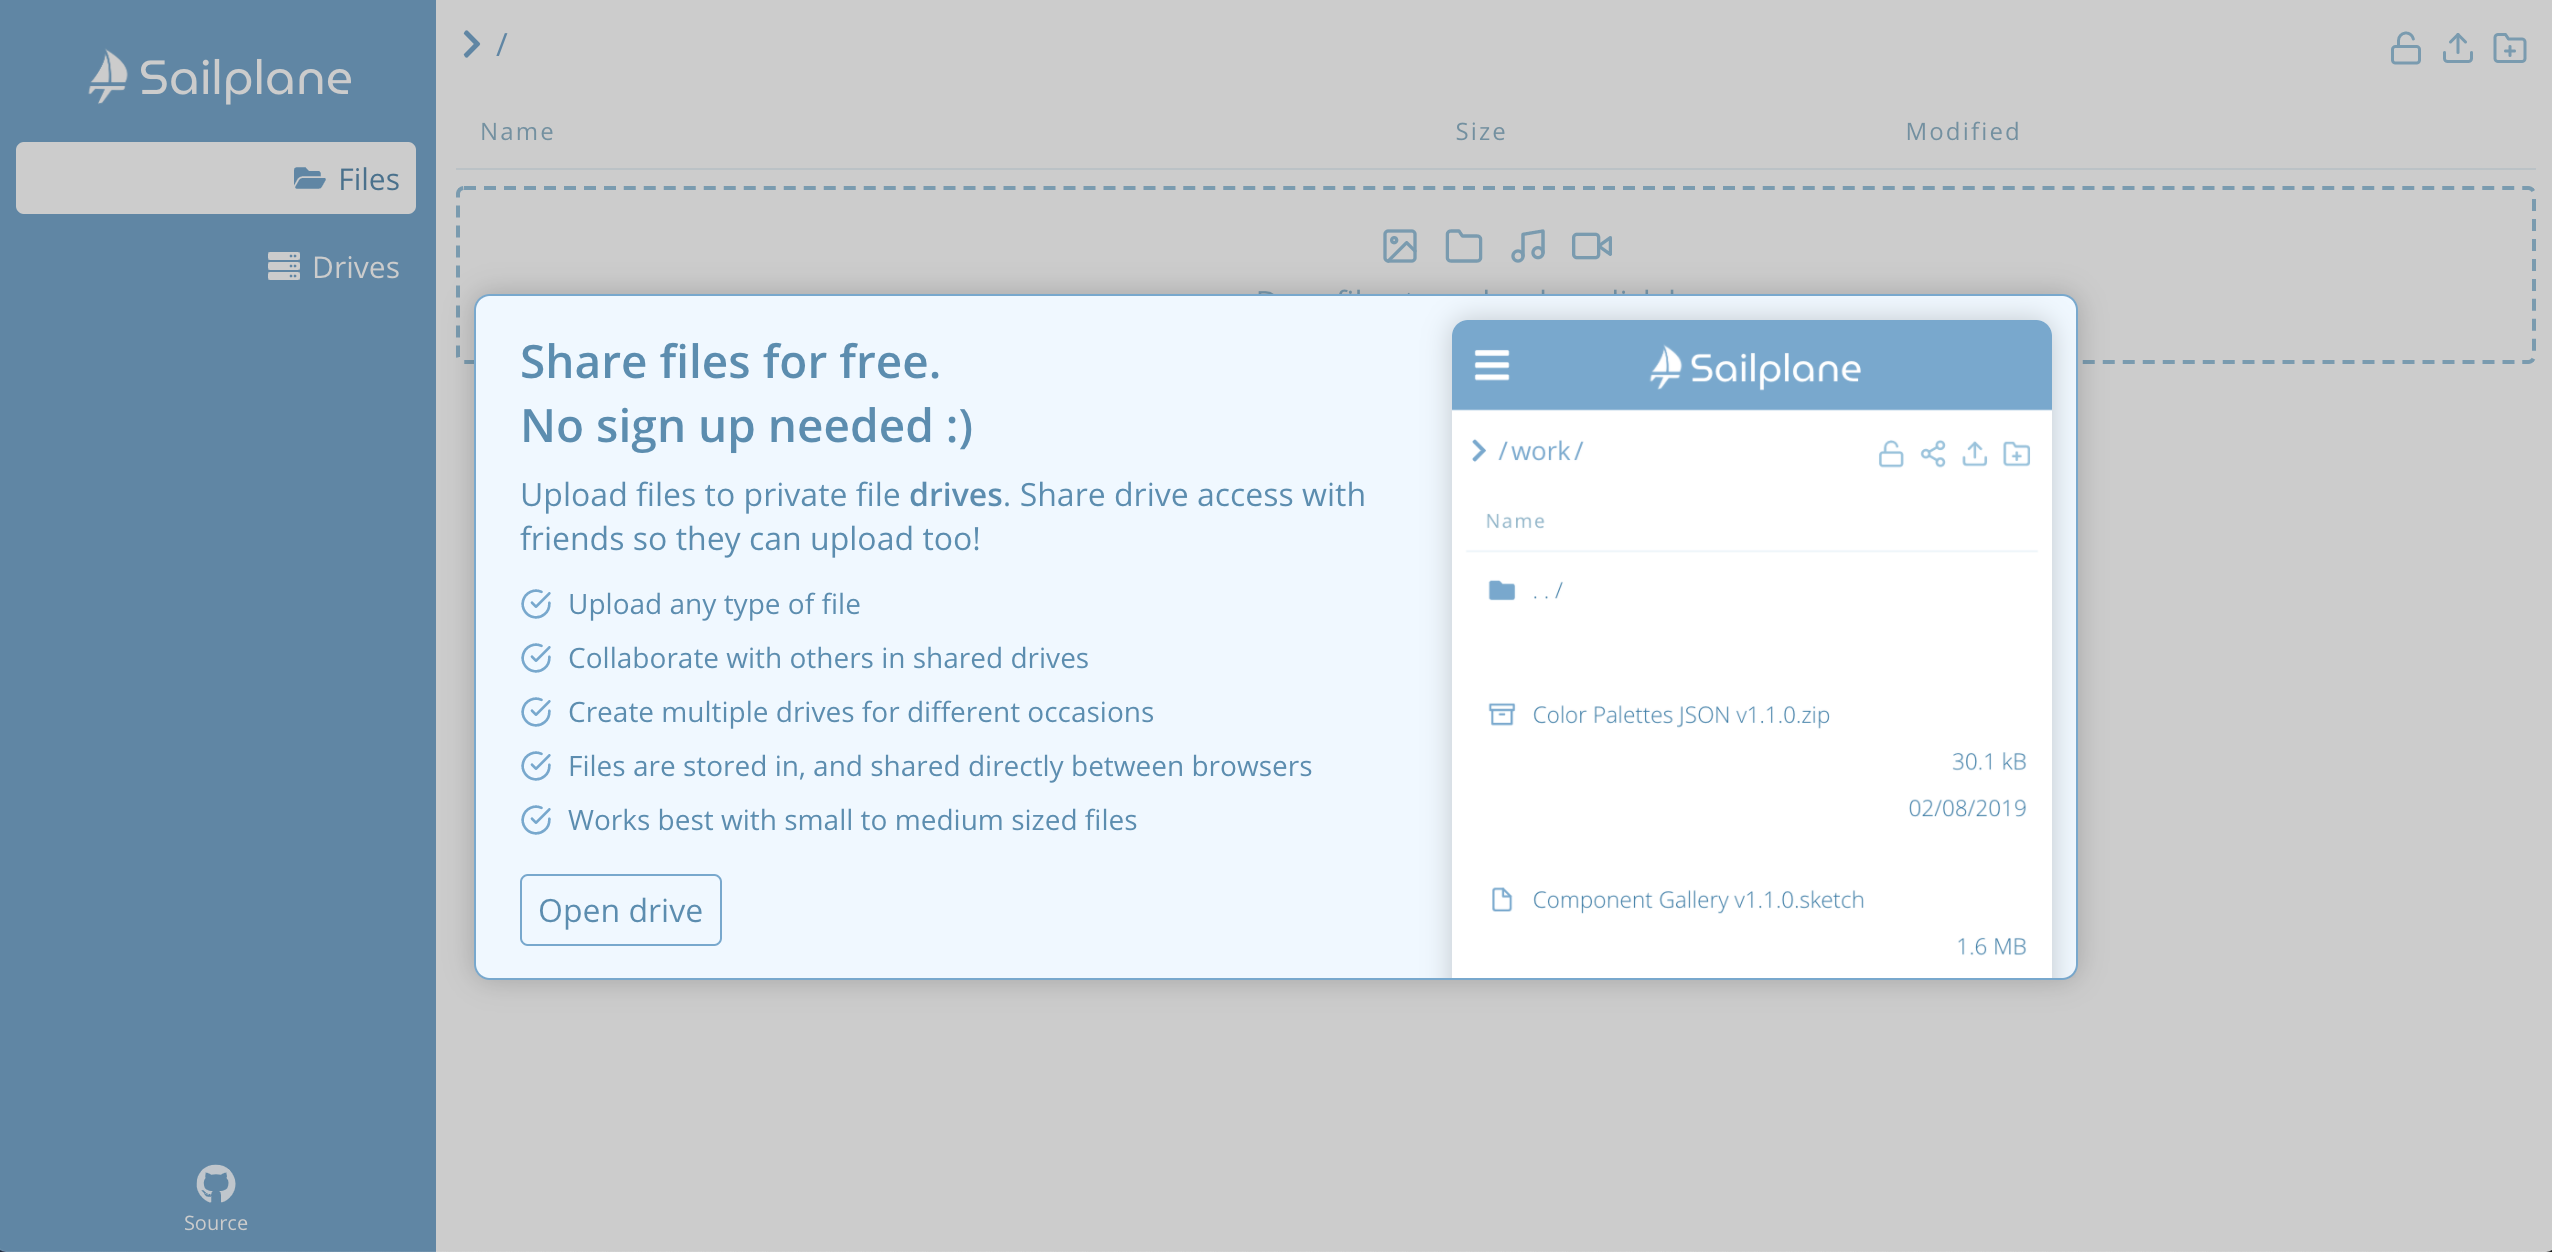
\includegraphics[width=\linewidth]{images/sailplane.png}
    \caption{Aplicación web de Sailplane}
    \label{fig:sailplaneweb}
\end{figure}

Sailplane ofrece una implementación de un nodo IPFS personalizado llamado
\\\textit{sailplane-node}\cite{Sailplanenode2023}, que expone una interfaz para interactuar directamente con el store.
Existe también una web que hace uso de este nodo y ofrece:
\begin{itemize}
    \item Un sistema de ficheros en el navegador basado en \textit{drives} (discos virtuales) compartidos.
    \item Un sistema de registro automático y autocontenido. Esto sirve para que la hora de compartir un drive este pueda
          ver los usuarios con los que puede compartirlo.
\end{itemize}

\begin{figure}[H]
    \centering
    \small
    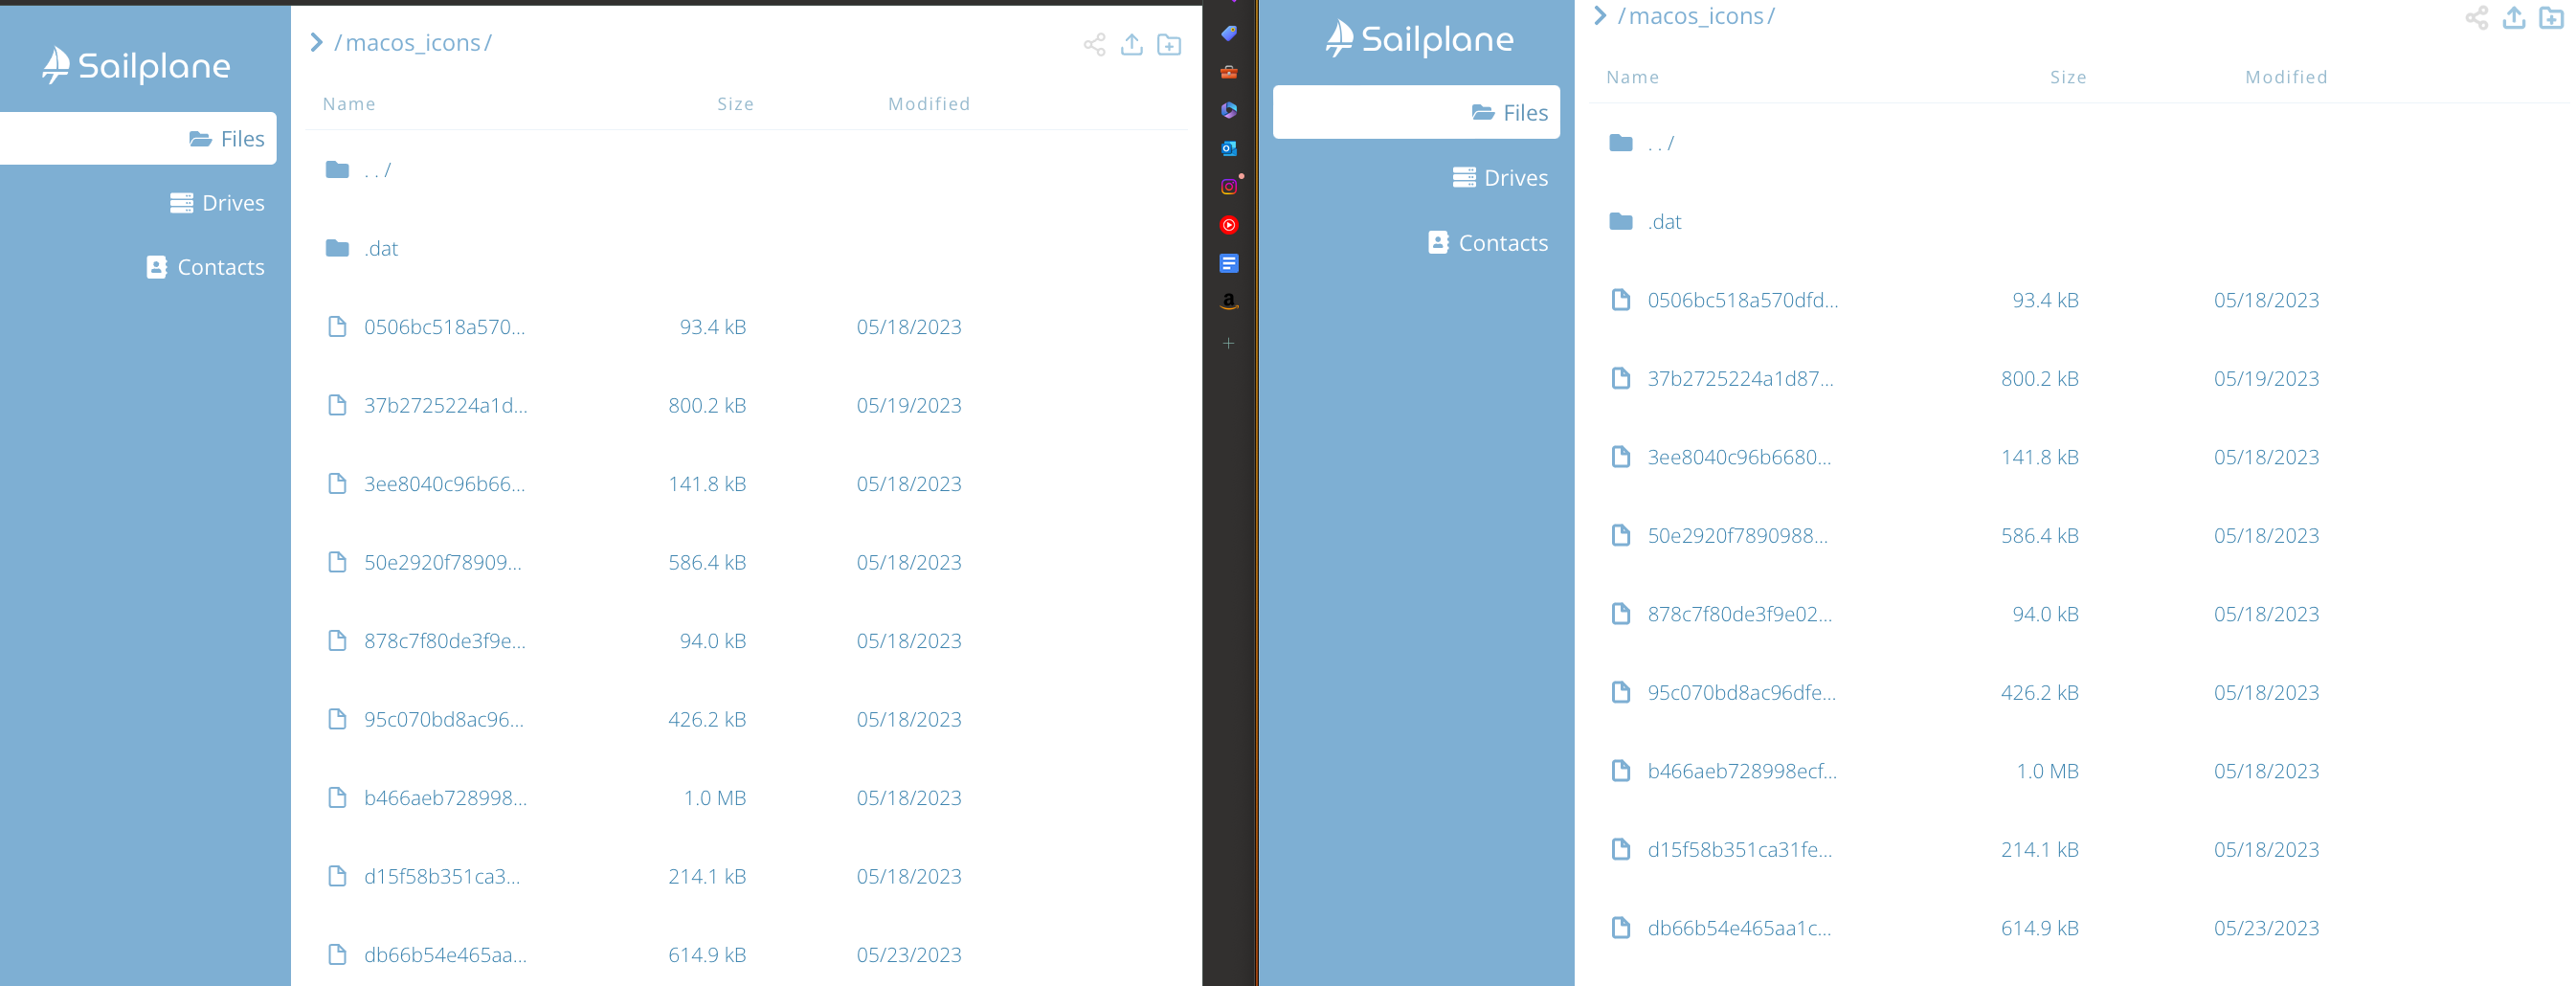
\includegraphics[width=\linewidth]{images/saiplanesynced.png}
    \caption{Dos nodos Sailplane sincronizando el el mismo drive}
    \label{fig:sailplanewebsync}
\end{figure}

Lo que más destaca de Sailplane es  la implementación de un sistema de ficheros montado sobre OrbitDB.
Esto es algo que se explorará más adelante en la el capítulo \ref{chap:7trabajosfuturos}: '\nameref{chap:7trabajosfuturos}'.
El uso de OrbitDB para un sistema de registro automático y autocontenido es algo que también se ha implementado en la propuesta, aunque como se ha
comentado previamente, el descubrimiento de este proyecto ocurrió ya habiendo desarrollado esta característica.

\section{Fileverse}
Fileverse es una plataforma de almacenamiento que se integra con IPFS y que permite guardar, compartir y acceder a archivos desde cualquier dispositivo.


Actualmente ofrece dos productos, ambos en formato de aplicación web:
\begin{itemize}
    \item Fileverse Solo: Una aplicación web para subir y compartir archivos sin autenticación. El usuario sube un archivo y recibe un enlace que puede compartir con otros usuarios. En la figura \ref{fig:fileverse} se puede observar un ejemplo de uso.
    \item Fileverse Portals: Una aplicación web que integra autenticación basada en blockchain. Es un espacio de trabajo para la gestión de archivos sobre blochain (e IPFS) y la creación de contenido. Está en fase de pruebas y no se puede acceder.
\end{itemize}
\begin{figure}[H]
    \centering
    \small
    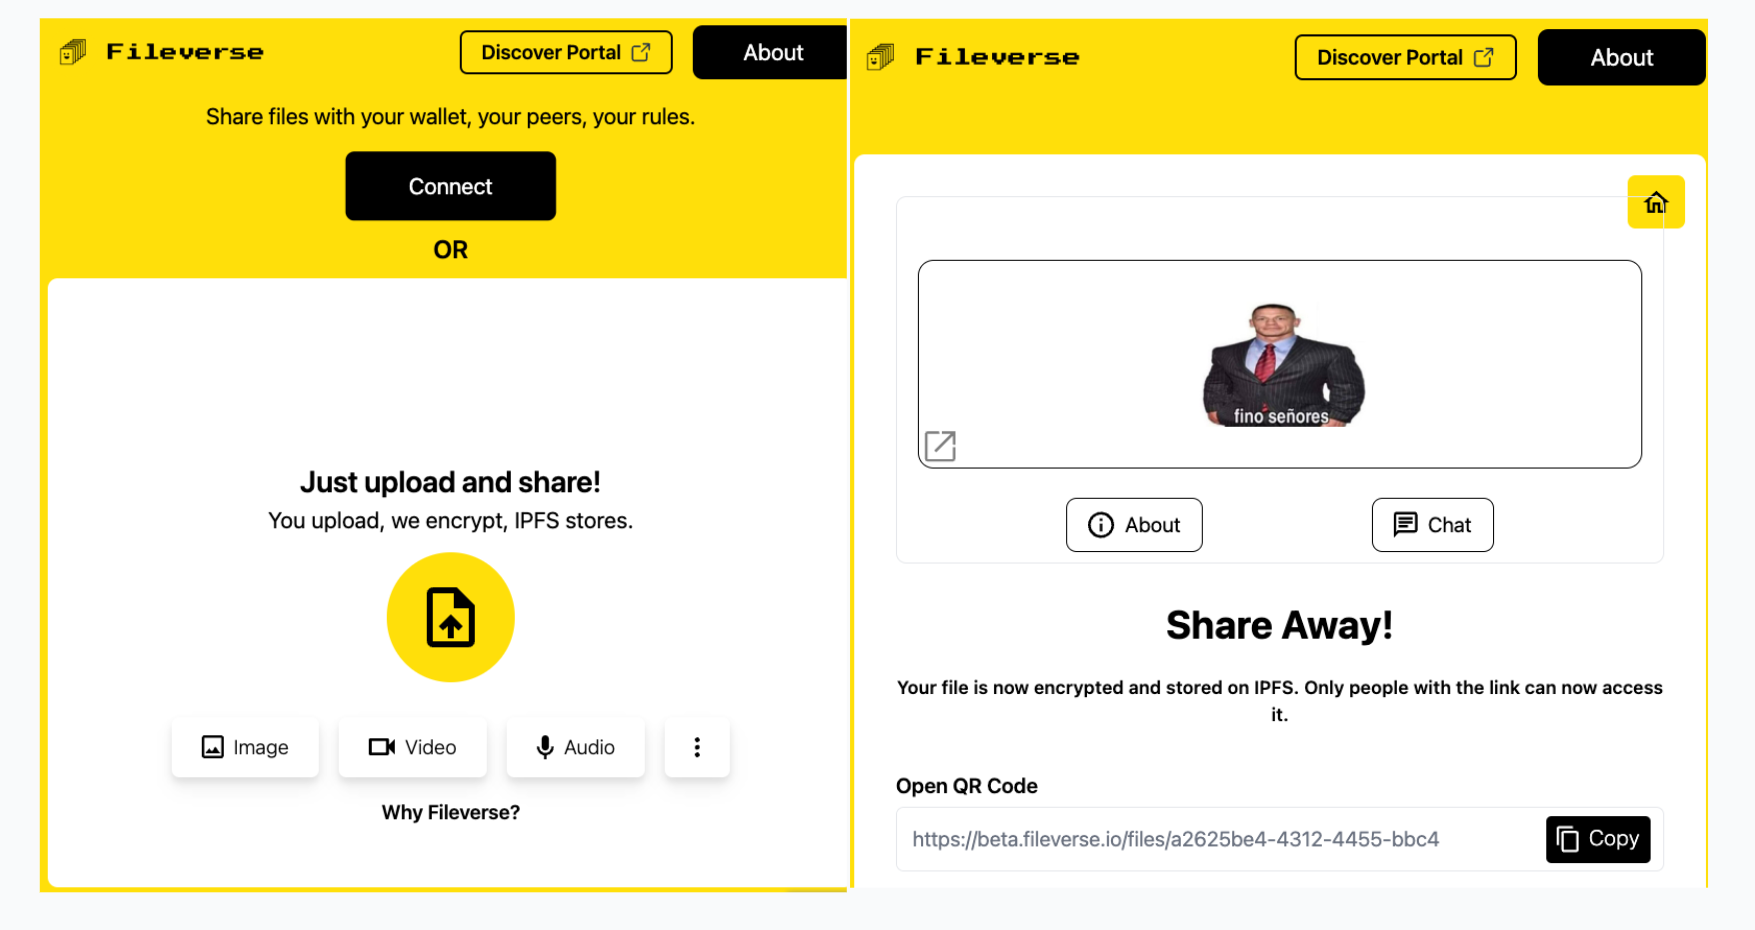
\includegraphics[width=\linewidth]{images/fileverse.png}
    \caption{Aplicación web de Fileverse para subir archivos}
    \label{fig:fileverse}
\end{figure}

El servicio que ofrece Fileverse Solo es muy simple: el usuario sube un archivo y recibe un enlace que puede pasar a otras personas para descargar dicho archivo.
Esta caso de uso es muy similar al que se propone en este proyecto, aunque con algunas diferencias. El uso de una
aplicación web resulta más sencillo que una línea de comandos, pero no integra cuentas de usuario ni formas de acceder o gestionar comparticiones pasadas.


\section{Conclusión}

Como se puede observar en este capítulo existen varias implementaciones de sistemas de almacenamiento y compartición de
archivos basadas en IPFS. Como opinión personal, ninguna presenta un servicio comparable al de los grandes
proveedores centralizados de almacenamiento en la nube. Tanto en términos de facilidad de uso, como de funcionalidades y
fiabilidad.

Esto se debe a que detrás de estos servicios hay una gran infraestructura e inversión que no es comparable a estos proyectos
que tienen un carácter más experimental, investigativo y proviene de equipos de desarrollo mucho más limitados. Aún así, estos proyectos son un buen ejemplo de lo que se puede lograr con IPFS y
han sido de gran ayuda a la hora de realizar este proyecto, en particular Sailplane y Peergos.
